\documentclass[addpoints, 12pt]{exam}%, answers]
\usepackage[utf8]{inputenc}
\usepackage[T1]{fontenc}

\usepackage{lmodern}
\usepackage{arydshln}
\usepackage[margin=2cm]{geometry}

\usepackage{enumitem}

\usepackage{enumerate}
\usepackage{breqn}
\usepackage{parskip}

\usepackage{amsmath, amsthm, amsfonts, amssymb}
\usepackage{graphicx}
\usepackage{tikz}
\usetikzlibrary{arrows,calc,patterns}
\usepackage{pgfplots}
\pgfplotsset{compat=newest}
\usepackage{url}
\usepackage{multicol}
\usepackage{thmtools}

\usepackage{caption}
\usepackage{subcaption}

\usepackage{pifont}

% MATH commands
\newcommand{\bC}{\mathbb{C}}
\newcommand{\bR}{\mathbb{R}}
\newcommand{\bN}{\mathbb{N}}
\newcommand{\bZ}{\mathbb{Z}}
\newcommand{\bT}{\mathbb{T}}
\newcommand{\bD}{\mathbb{D}}

\DeclareMathOperator{\dom}{dom}


\newcommand{\spc}{\vspace*{0.5cm}}
\CorrectChoiceEmphasis{\color{red}}

\begin{document}
\noindent \hrulefill \\
	MATH-241 Calculus I \hfill Created by Rukiyah Walker\\
	Homework 4 \hfill Spring 2023\\ \vspace*{-1cm}
 
	\noindent\hrulefill

\qformat{\rule{0.3\textwidth}{.4pt} \begin{large}{\textsc{Question}} \thequestion \end{large} \hspace*{0.2cm} \hrulefill \hspace*{0.1cm} \textbf{(\totalpoints\hspace*{0.1cm} pts)}}

\begin{questions}

\vspace*{1cm}

\question[1]

We use the Intermediate Value Theorem to: 

\begin{choices}
\choice To show that a function is continuous.
\CorrectChoice To show that for a continuous function $f(x)$, a solution to $f(x) = 0$ exists.
\choice To show that a function is discontinuous. 
\choice To show that $\lim_{x \to a} f(x)$ does not exist.
\end{choices}

\spc

\question[1]

What do we need to check in order to use the Intermediate Value Theorem?

\begin{choices}
\choice Our function $f(x)$ is continuous on the closed interval $[a, b]$.
\choice $f(a) \neq f(b)$.
\choice $f(a) \leq N \leq f(b)$, where $N$ is some number. 
\CorrectChoice All of the above.
\end{choices}

\spc

\question[1]

The derivative of a function $f$ is:

\begin{choices}
\CorrectChoice $f'(a) = \lim_{h \to 0} \frac{f(a + h) - f(a)}{h}$
\choice The value $a$, when $f(a) = 0$.
\choice When the limit of a function does not exist.
\choice The value at which a function is discontinuous. 
\end{choices}

\spc

\question[1]
What is one interpretation of the average rate of change?

\begin{choices}
\choice Instantaneous velocity. 
\choice $f'(a) = \lim_{h \to 0} \frac{f(a + h) - f(a)}{h}$
\CorrectChoice The average change in position with respect to time. 
\choice The derivative of a function $f$.
\end{choices}

\newpage

\question[1]
What is the instantaneous rate of change?

\begin{choices}
\CorrectChoice The derivative of a function $f$.
\choice Acceleration.
\choice The point at which a function is discontinuous. 
\choice When a function $f(x) = 0$.
\end{choices}

\spc

\question[1]
The derivative of a function $f$ is equal to 0 when:

\begin{choices}
\choice The graph of the function crosses the $x$-axis.
\CorrectChoice When the slope of the tangent line is 0.
\choice At the point $x = 0$.
\choice The derivative does not exist.
\end{choices}

\spc

\question[1]
What does $\frac{dy}{dx}\textbar_{x = a} = f'(a)$ mean?

\begin{choices}
\choice The average rate of change is equal to $f'(a)$.
\choice The derivative of $y$ divided by the derivative of $x$ is equal to $f'(a)$.
\choice $f(x) = f'(a)$ when $x = a$.
\CorrectChoice The derivative of a function $f$ at the point $x = a$ is equal to $f'(a)$.
\end{choices}

\spc

\question[1]
Suppose we have a function $f$ that represents the position of a particle. The acceleration of the particle can be represented by: 

\begin{choices}
\choice The velocity.
\choice $f'(x)$.
\CorrectChoice The second derivative of the function.
\choice The instantaneous rate of change.
\end{choices}

\newpage

\question[1]
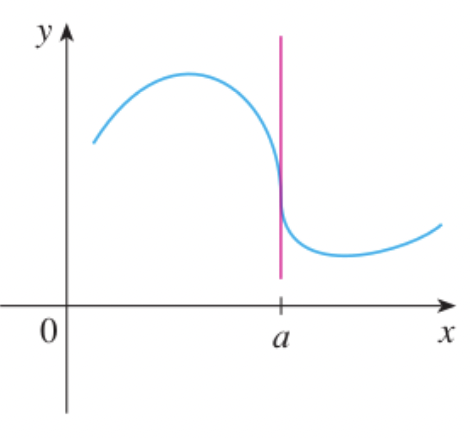
\includegraphics[width=0.4\textwidth]{Hw4graph.png}

Is the function, represented by the graph above, differentiable? Why?

\begin{choices}
\CorrectChoice No, since the slope of the tangent line is equal to $\pm \infty$.
\choice Yes, since $\lim_{x \to a^-} f(x) = \lim_{x \to a^+} f(x)$.
\choice Yes, since there is no jump discontinuity.
\choice No, since $\lim_{x \to a} f(x) = 0$
\end{choices}

\spc

\question[1]
Suppose we have the function $f(x) = x^3 - x^2$.

Using the power and difference rules for derivatives, what is $f'(x)$?

\begin{choices}
\choice $3x^3 - 2x^2$
\CorrectChoice $3x^2 - 2x$
\choice $3x - 2x$
\choice $3x^4 - 2x^3$
\end{choices}

\spc

\end{questions}

\end{document}